\documentclass[a4paper,11pt]{article}
\usepackage{lmodern}
\renewcommand*\familydefault{\sfdefault}
\usepackage{sfmath}
\usepackage[utf8]{inputenc}
\usepackage[T1]{fontenc}
\usepackage[italian]{babel}
\usepackage{indentfirst}
\usepackage{graphicx}
\usepackage{tikz}
\usepackage{wrapfig}
\usepackage{enumitem}
\usepackage[left=2cm, right=2cm, bottom=3cm]{geometry}
\usepackage{textcomp}
\usepackage{xstring}
\IfFileExists{siunitx.sty}{
 \usepackage[group-separator={\,}]{siunitx}
}{
 \newcommand{\num}[1]{#1}
}
\frenchspacing

% Macro varie...
\input{glyphtounicode}
\pdfglyphtounicode{visiblespace}{3000}
\pdfglyphtounicode{blank}{3000}
\pdfglyphtounicode{visualspace}{3000}
\pdfglyphtounicode{uni2423}{3000}
\pdfgentounicode=1

\newcommand{\formatline}[1]{
 \IfBeginWith{#1}{ }{
  \StrGobbleLeft{#1}{1}[\tmp]
  \formatline{\tmp}
 }{
  \IfEndWith{#1}{ }{
   \StrGobbleRight{#1}{1}[\tmp]
   \formatline{\tmp}
  }{
   \StrSubstitute{#1}{ }{\textcolor{white}{\char32}}
  }
 }
}

\newcommand{\formatlines}[1]{
 \IfSubStr{#1}{\par}{
  \StrCut{#1}{\par}{\first}{\rest}
  \formatline{\first}
  \par
  \formatlines{\rest}
 }{
  \formatline{#1}
 }
}

\newcommand{\formatfile}[1]{
 \tt \small \formatlines{#1}
}

\newcommand{\file}[1]{\texttt{#1}}
\renewcommand{\arraystretch}{1.3}
\newcommand{\esempio}[2]{
\noindent\begin{minipage}{\textwidth}
\begin{tabular}{|p{11cm}|p{5cm}|}
	\hline
	\textbf{File \file{input.txt}} & \textbf{File \file{output.txt}}\\
	\hline
	\formatfile{#1} &
	\formatfile{#2} \\
	\hline
\end{tabular}
\end{minipage}
}

\newcommand{\sezionetesto}[1]{
    \section*{#1}
}

\newcommand*\circled[1]{\tikz[baseline=(char.base)]{
		\node[shape=circle,draw,inner sep=2pt] (char) {#1};}}

\newcommand{\gara}{Olimpiadi Italiane di Informatica - Selezioni Territoriali 2014}

%%%%% I seguenti campi verranno sovrascritti dall'\include{nomebreve} %%%%%
\newcommand{\nomebreve}{}
\newcommand{\titolo}{}
\newcommand{\difficolta}{}

% Modificare a proprio piacimento:
\newcommand{\introduzione}{
    \noindent{\Large \gara{}}

    \vspace{0.5cm}
    \noindent{\Huge \textbf \titolo{}~(\texttt{\nomebreve{}})}
    \vspace{0.2cm}\\
    \noindent{\difficolta{}}\\
}

\begin{document}

\renewcommand{\nomebreve}{mojito}
\renewcommand{\titolo}{Giochiamo con Mojito}
\renewcommand{\difficolta}{\normalsize \textsc{[Difficoltà D=2]}}

{ % begin hack

\introduzione{}

\begin{wrapfigure}{r}{3cm}
	\begin{center}
		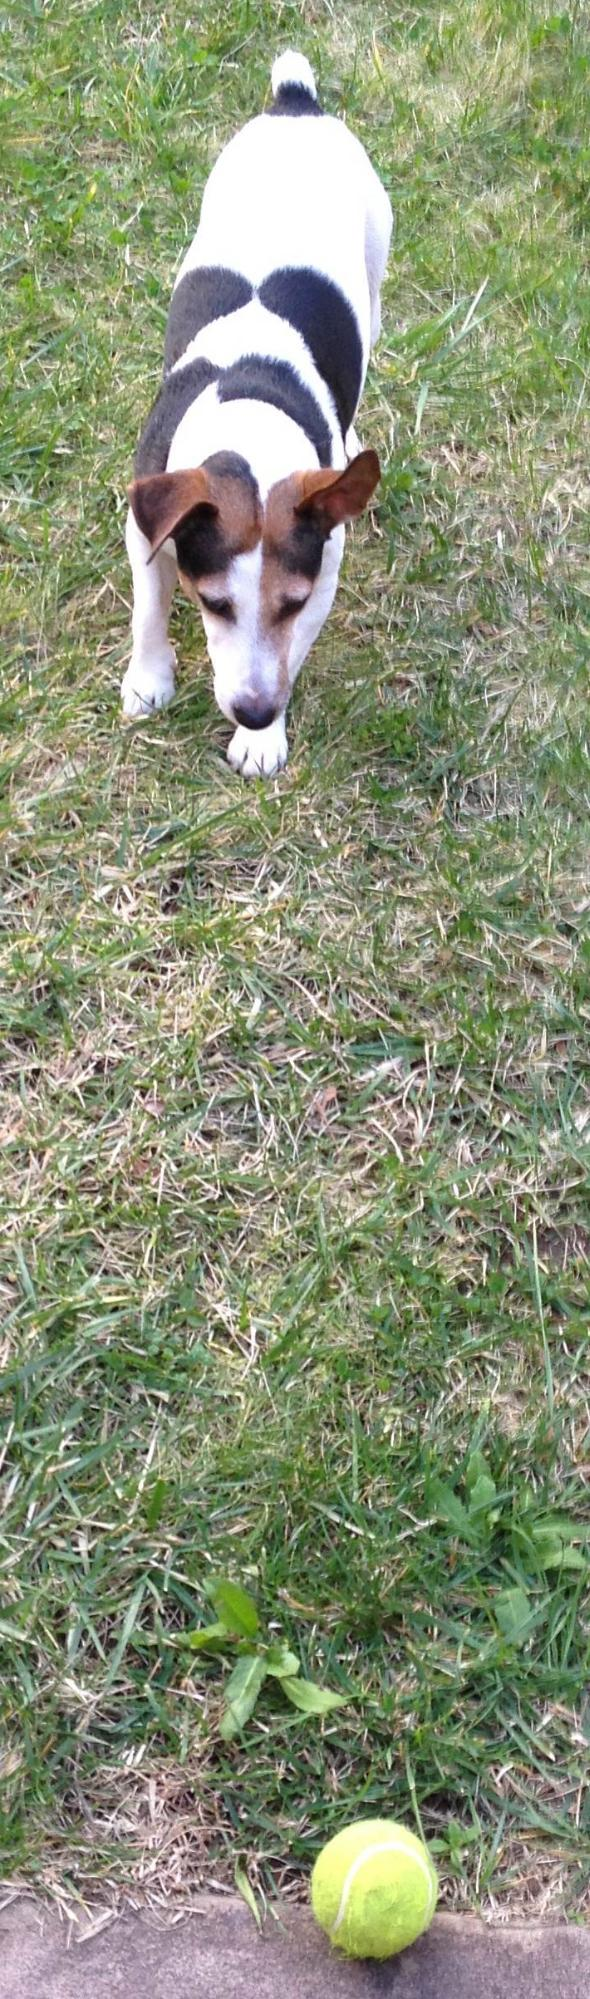
\includegraphics[width=2cm]{image00.jpg}
	\end{center}
\end{wrapfigure}

Mojito, il jackrussell di Monica, è ormai diventato la mascotte dei
Probabili Olimpici, i ragazzi che sono candidati a rappresentare
l’Italia alle Olimpiadi Internazionali di Informatica 2014 a Taipei,
Taiwan. Negli allenamenti a Volterra, Mojito gioca a palla con i
ragazzi nel prato: lui porta la pallina al ragazzo più vicino che la
calcia via; a quel punto Mojito rincorre la palla, l’acchiappa e la
porta di nuovo al ragazzo che ha più vicino\dots e così via!

Possiamo rappresentare questo gioco con una griglia: supponendo di
avere tre ragazzi che giocano con Mojito, rappresentiamo la loro
posizione nella griglia, rispettivamente, con R1, R2 e R3. Tutti i
ragazzi sono piuttosto metodici, e ogni volta che tirano la palla
questa finisce sempre nella stessa posizione (a seconda di chi tira!):
sulla griglia indichiamo con P1 il punto in cui finisce la palla
tirata da R1, P2 il punto in cui finisce la palla tirata da R2,
ecc\dots La posizione iniziale di Mojito, con la palla, è
rappresentata nella griglia da una M. Mojito misura la distanza come
il minimo numero di spostamenti orizzontali e/o verticali per andare
da una casella a un’altra.

\begin{center}
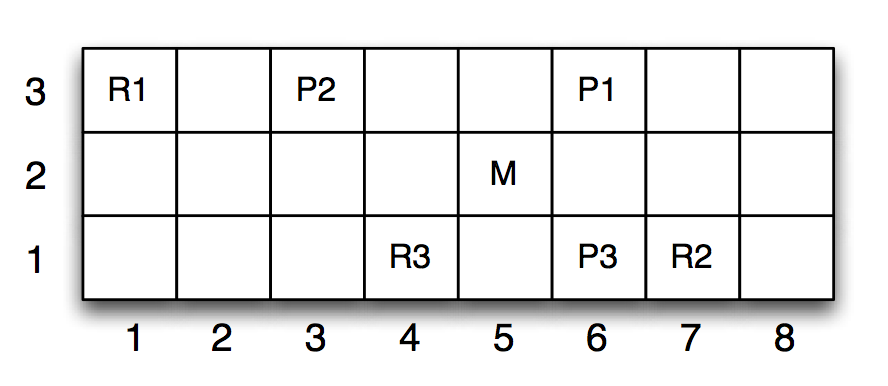
\includegraphics{mojito.png}
\end{center}

} % end hack

Per esempio, consideriamo la griglia qui sopra, di dimensione $8
\times 3$. All’inizio Mojito si trova, insieme con la palla, nella
casella $(5,2)$; il ragazzo più vicino è R3, nella posizione $(4,1)$,
che dista due caselle da lui; il gioco inizia:

\begin{itemize}[noitemsep]
  \item Mojito porta la palla a R3, che la tira nella casella $(6,1)$;
  \item a questo punto Mojito, presa la palla, la porta a R2, nella
    casella $(7,1)$, che è il più vicino a lui; da qui la palla viene
    tirata nella casella $(3,3)$;
  \item Mojito recupera la palla e la porta a R1, nella casella
    $(1,3)$; R1 tira la palla nella casella $(6,3)$;
  \item da qui in poi saranno solo R1 e R2 a giocare, visto che quando
    tira R1 poi Mojito porta la palla a R2 e viceversa.
\end{itemize}

Notiamo che, nel caso appena descritto, tutti e tre i ragazzi hanno
giocato (anche se R3 ha toccato palla solo una volta). Se Mojito ha
due o più ragazzi alla stessa distanza, sceglie quello che ha la
coordinata $X$ (orizzontale) minore e, se ve ne sono due o più con lo
stesso valore, tra questi sceglie quello che ha la coordinata $Y$
(verticale) minore. Mojito è molto concentrato sulla palla, e non
riesce a ricordarsi se tutti i ragazzi l’hanno tirata. Il vostro
compito è quello di scrivere un programma che calcoli il numero di
ragazzi che lanciano la palla almeno una volta!

\sezionetesto{Dati di input}
Il file \verb'input.txt' è composto da $3+N$ righe. La prima riga
contiene due interi positivi $X$ e $Y$: le dimensioni della
griglia. La seconda riga contiene una coppia di interi positivi: le
coordinate della posizione iniziale di Mojito con la palla. La terza
riga contiene $N$, il numero di ragazzi che giocano con Mojito. Ognuna
delle successive $N$ righe contiene due coppie di interi: le
coordinate dell’$i$-esimo ragazzo (prima coppia di interi) e le
coordinate di dove l’$i$-esimo ragazzo tirerà la palla.

\sezionetesto{Dati di output}
Il file \verb'output.txt' è composto da una sola riga contenente un
solo intero non negativo: il numero di ragazzi che giocano con Mojito,
ovvero il numero di ragazzi che tirano la palla almeno una volta, a
partire dalla posizione iniziale di Mojito.

% Assunzioni
\sezionetesto{Assunzioni}
\begin{itemize}[nolistsep, noitemsep]
  \item $1 \le X,Y,N \le 100$
  \item Le coordinate della griglia vanno da $1$ a $X$ e da $1$ a $Y$
    (inclusi).
  \item Tutte le posizioni nel file di input sono distinte: non ci
    possono essere due ragazzi nella stessa casella, non ci sono due
    ragazzi che tirano nella stessa casella, nessun ragazzo tira nella
    casella dove c’è un altro ragazzo.
  \item Mojito, inizialmente, è in una casella non occupata da nessun
    ragazzo e dove nessun ragazzo tira la palla.
  \item Mojito, piccolo com’è, riesce agevolmente a passare tra le
    gambe dei ragazzi; non viene quindi ostacolato nel suo movimento
    da ragazzi presenti in una cella tra lui e la palla.
\end{itemize}

% Esempi
\sezionetesto{Esempio di input/output}
\esempio{
5 3

3 3

2

4 3 5 3

5 1 1 1
}{1}

\esempio{
8 3

5 2

3

1 3 6 3

7 1 3 3

4 1 6 1
}{3}


\end{document}
